\section{Appendix on latent-space control}\label{sec:apx-con:latent_space_control}
Below, we present supplementary results for the model-based, latent-space control on the two-segment, piecewise constant curvature soft robot (\emph{PCC-NS-2}).

\begin{figure}[ht]
    \centering
    \subfigure[Configuration $q(t) \in \mathbb{R}^2$]{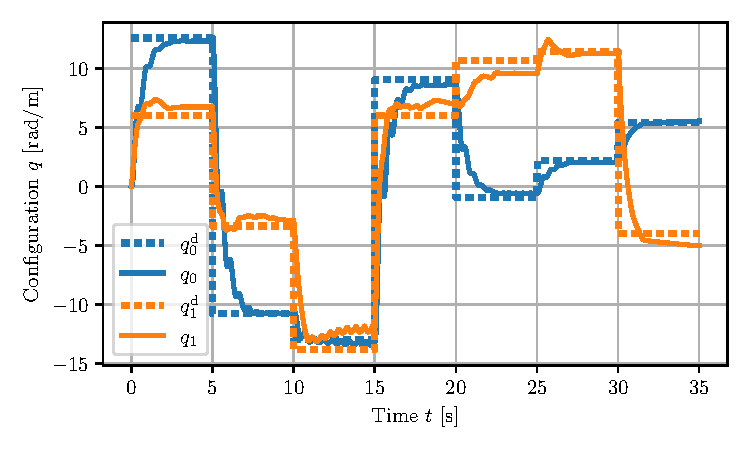
\includegraphics[width=0.49\columnwidth, trim={5, 10, 5, 5}]{con/figures/results/control/pcc_ns-2/mech_node_psatid/setpoint_control_sequence_q.pdf}}
    \subfigure[Latent representation $z(t) \in \mathbb{R}^2$]{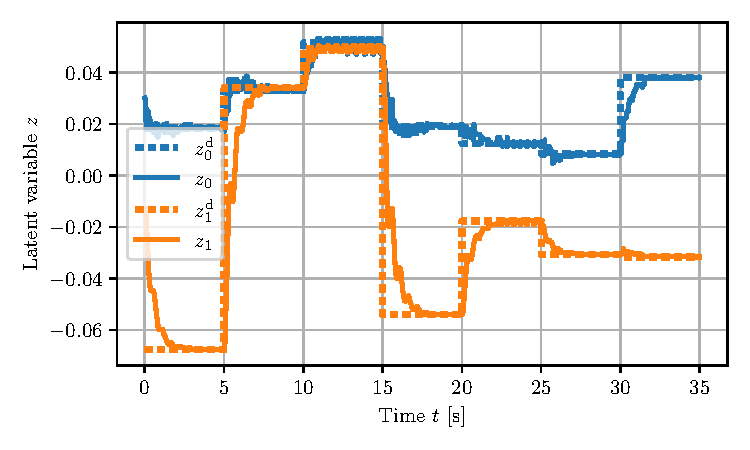
\includegraphics[width=0.49\columnwidth, trim={5, 10, 5, 5}]{con/figures/results/control/pcc_ns-2/mech_node_psatid/setpoint_control_sequence_z.pdf}}\\
    \subfigure[Control input $u(t) \in \mathbb{R}^2$]{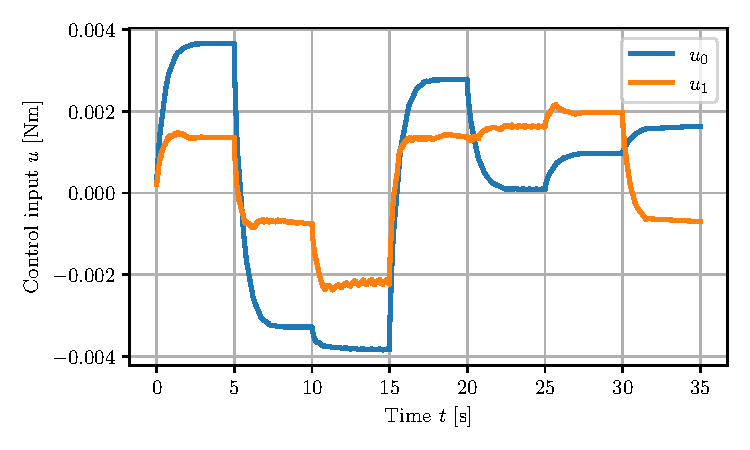
\includegraphics[width=0.49\columnwidth, trim={5, 10, 5, 5}]{con/figures/results/control/pcc_ns-2/mech_node_psatid/setpoint_control_sequence_u.pdf}}
    \caption{Latent-space control of a continuum soft robot (simulated using two \gls{PCC} segments) following a sequence of setpoints with a pure \textbf{P-satI-D} feedback controller operating in a 2D latent space learned with the \textbf{MECH-NODE} model. The \gls{CON} model weights are initialized using a \textbf{random seed of 0}.
    The dotted and solid lines show the reference and actual values, respectively.
    For each setpoint, we randomly sample a desired shape $q^\mathrm{d}$ and render the corresponding image $o^\mathrm{d}$. This image is then encoded to a target latent $z^\mathrm{d}$. The controller then computes a latent-space torque $F^\mathrm{d}$, which is decoded to an input $u$. Finally, we provide this input to the simulator, which performs a roll-out of the closed-loop dynamics.
    Important: The robot's configuration (i.e., the first-principle, minimal-order state) is solely used for generating a target image and simulating the closed-loop system. 
    }\label{fig:apx-con:control:pcc_ns-2:mech_node_psatid_results}
\end{figure}


\begin{figure}[ht]
    \centering
    \subfigure[Configuration $q(t) \in \mathbb{R}^2$]{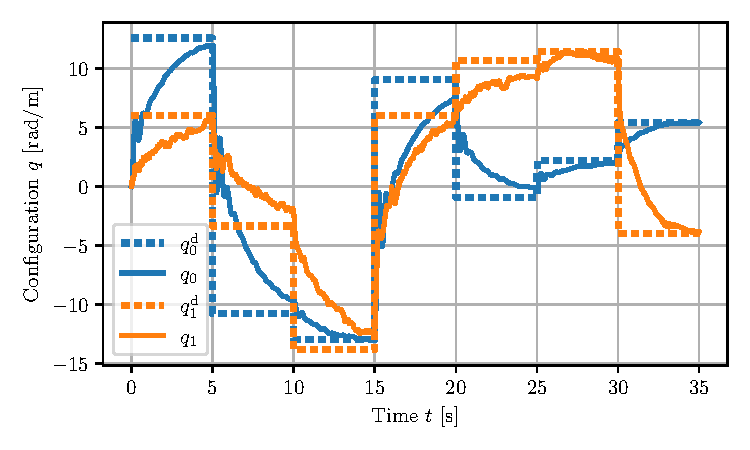
\includegraphics[width=0.49\columnwidth, trim={5, 10, 5, 5}]{con/figures/results/control/pcc_ns-2/con_psatid/setpoint_control_sequence_q.pdf}}
    \subfigure[Latent representation $z(t) \in \mathbb{R}^2$]{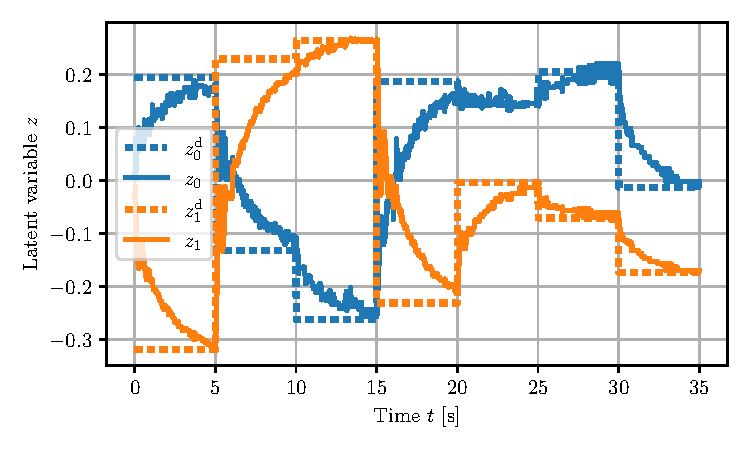
\includegraphics[width=0.49\columnwidth, trim={5, 10, 5, 5}]{con/figures/results/control/pcc_ns-2/con_psatid/setpoint_control_sequence_z.pdf}}\\
    \subfigure[Control input $u(t) \in \mathbb{R}^2$]{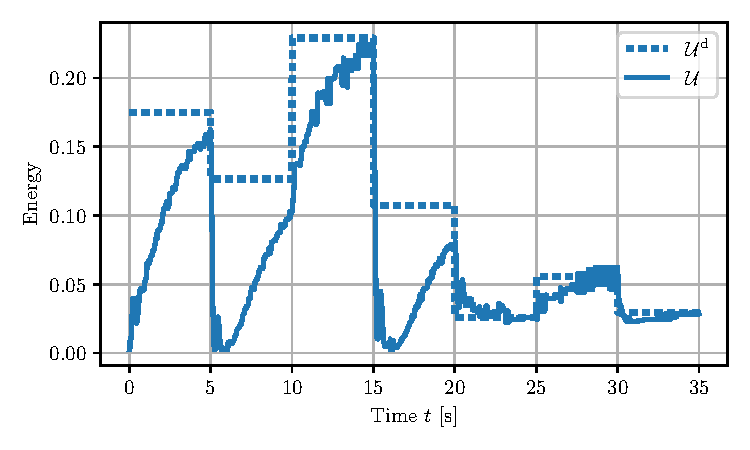
\includegraphics[width=0.49\columnwidth, trim={5, 10, 5, 5}]{con/figures/results/control/pcc_ns-2/con_psatid/setpoint_control_sequence_u.pdf}}
    \subfigure[Potential energy $U(t) \in \mathbb{R}$]{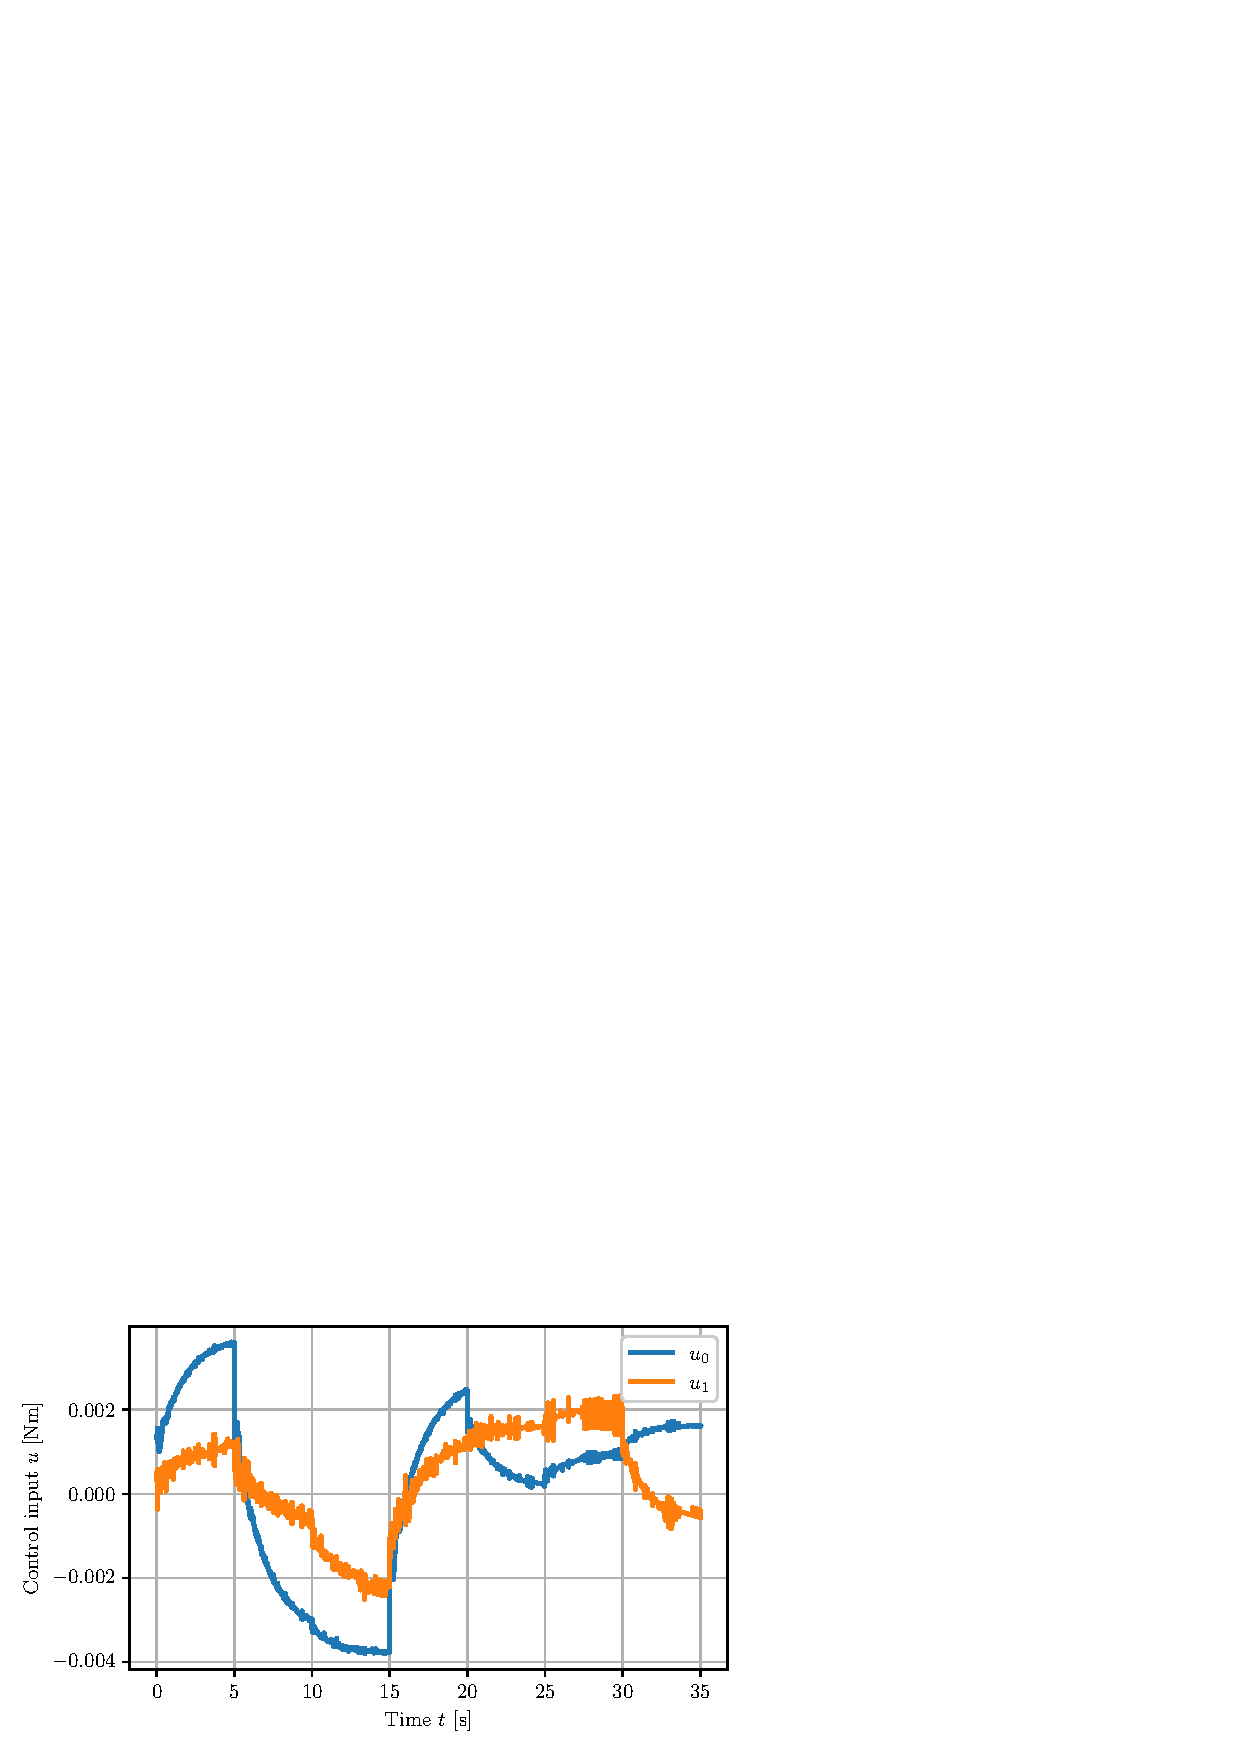
\includegraphics[width=0.49\columnwidth, trim={5, 10, 5, 5}]{con/figures/results/control/pcc_ns-2/con_psatid/setpoint_control_sequence_U.pdf}}
    \caption{Latent-space control of a continuum soft robot (simulated using two \gls{PCC} segments) following a sequence of setpoints with a pure \textbf{P-satI-D} feedback controller operating in a 2D latent space learned with the \textbf{\gls{CON}} model. The \gls{CON} model weights are initialized using a random seed of 0.
    The dotted and solid lines show the reference and actual values, respectively.
    For each setpoint, we randomly sample a desired shape $q^\mathrm{d}$ and render the corresponding image $o^\mathrm{d}$. This image is then encoded to a target latent $z^\mathrm{d}$. The controller then computes a latent-space torque $F^\mathrm{d}$, which is decoded to an input $u$. Finally, we provide this input to the simulator, which performs a roll-out of the closed-loop dynamics.
    Important: The robot's configuration (i.e., the first-principle, minimal-order state) is solely used for generating a target image and simulating the closed-loop system. 
    }\label{fig:apx-con:control:pcc_ns-2:con_PsatID_results}
\end{figure}


\begin{figure}[ht]
    \centering
    \subfigure[Configuration $q(t) \in \mathbb{R}^2$]{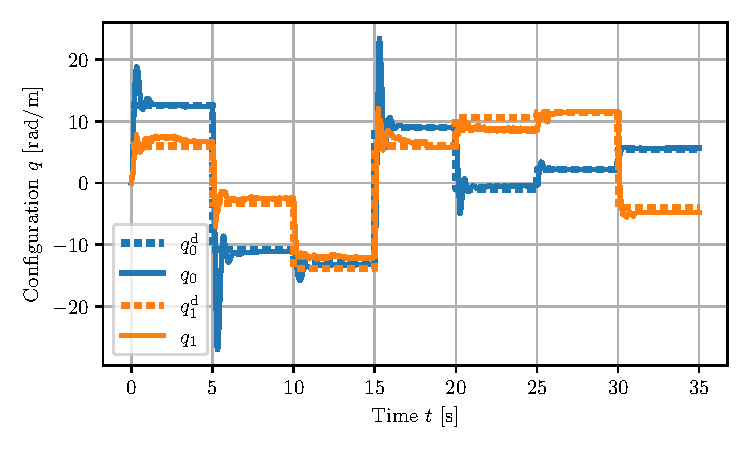
\includegraphics[width=0.49\columnwidth, trim={5, 10, 5, 5}]{con/figures/results/control/pcc_ns-2/con_psatid+ff/setpoint_control_sequence_q.pdf}}
    \subfigure[Latent representation $z(t) \in \mathbb{R}^2$]{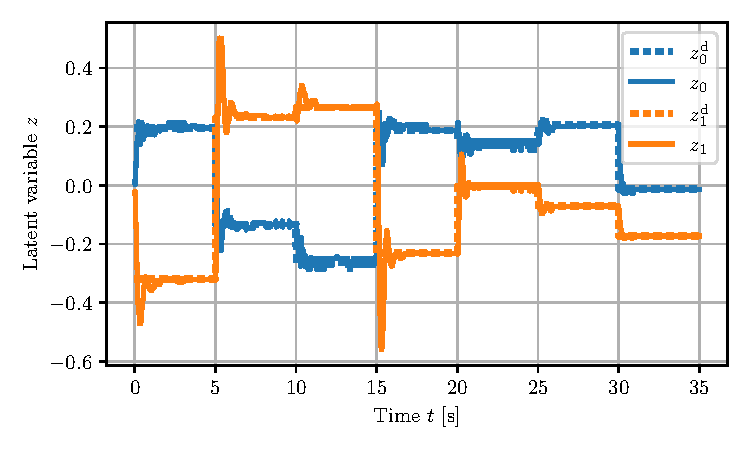
\includegraphics[width=0.49\columnwidth, trim={5, 10, 5, 5}]{con/figures/results/control/pcc_ns-2/con_psatid+ff/setpoint_control_sequence_z.pdf}}\\
    \subfigure[Control input $u(t) \in \mathbb{R}^2$]{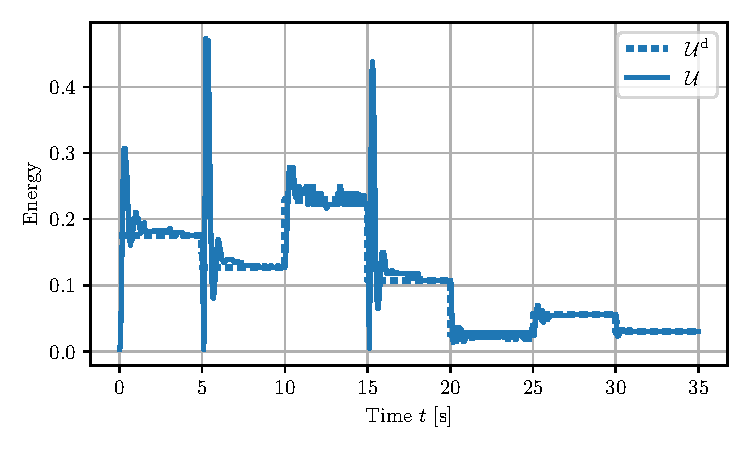
\includegraphics[width=0.49\columnwidth, trim={5, 10, 5, 5}]{con/figures/results/control/pcc_ns-2/con_psatid+ff/setpoint_control_sequence_u.pdf}}
    \subfigure[Potential energy $U(t) \in \mathbb{R}$]{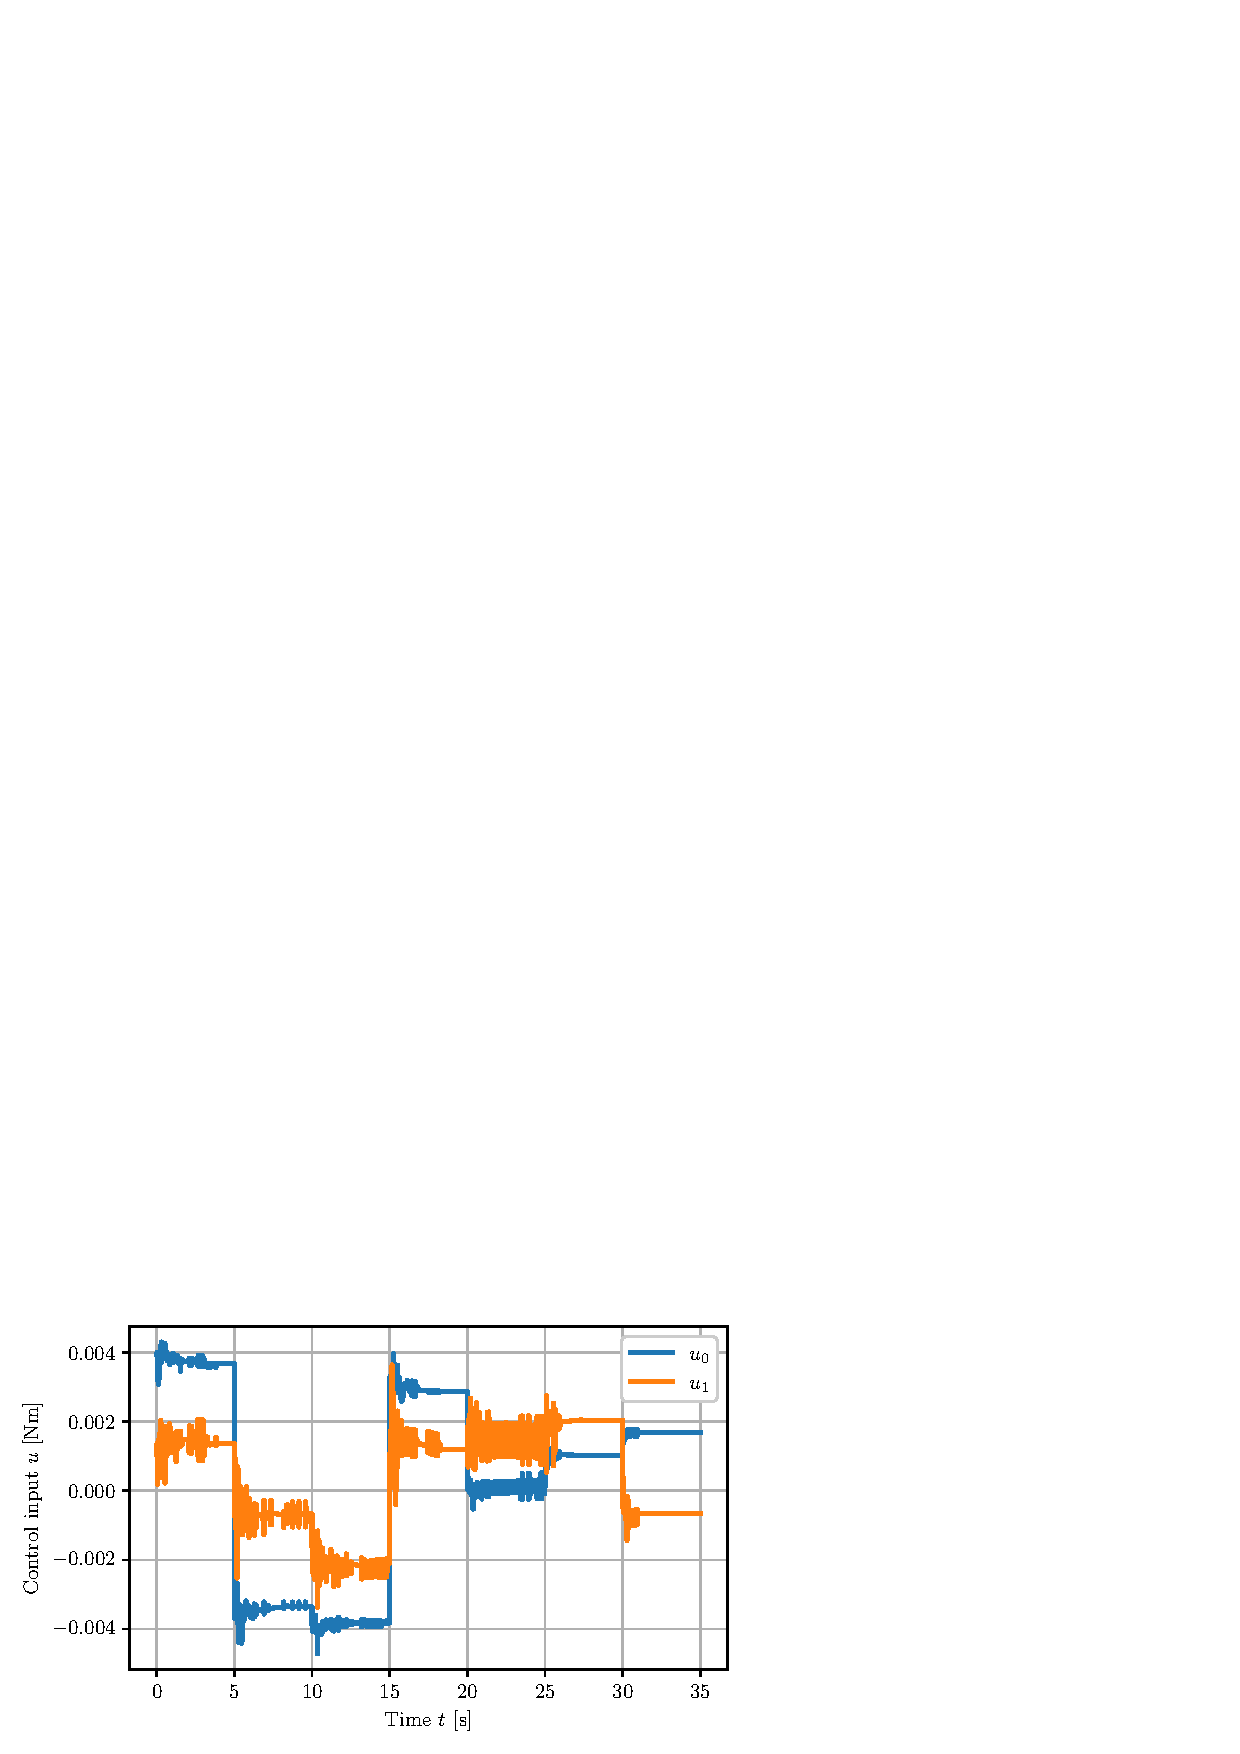
\includegraphics[width=0.49\columnwidth, trim={5, 10, 5, 5}]{con/figures/results/control/pcc_ns-2/con_psatid+ff/setpoint_control_sequence_U.pdf}}
    \caption{Latent-space control of a continuum soft robot (simulated using two \gls{PCC} segments) following a sequence of setpoints with a pure \textbf{P-satI-D+FF} feedback \& feedforward controller operating in a 2D latent space learned with the \textbf{\gls{CON}} model. The \gls{CON} model weights are initialized using a random seed of 0.
    The dotted and solid lines show the reference and actual values, respectively.
    For each setpoint, we randomly sample a desired shape $q^\mathrm{d}$ and render the corresponding image $o^\mathrm{d}$. This image is then encoded to a target latent $z^\mathrm{d}$. The controller then computes a latent-space torque $F^\mathrm{d}$, which is decoded to an input $u$. Finally, we provide this input to the simulator, which performs a roll-out of the closed-loop dynamics.
    Important: The robot's configuration (i.e., the first-principle, minimal-order state) is solely used for generating a target image and simulating the closed-loop system. 
    }\label{fig:apx-con:control:pcc_ns-2:con_PsatID+FF_results}
\end{figure}
